\begin{figure}[p]
  \begin{subfigure}[b]{.35\linewidth}
    \centering
    \begin{tikzpicture}
      \node[inner sep=0pt] (img) at (0, 0)
           {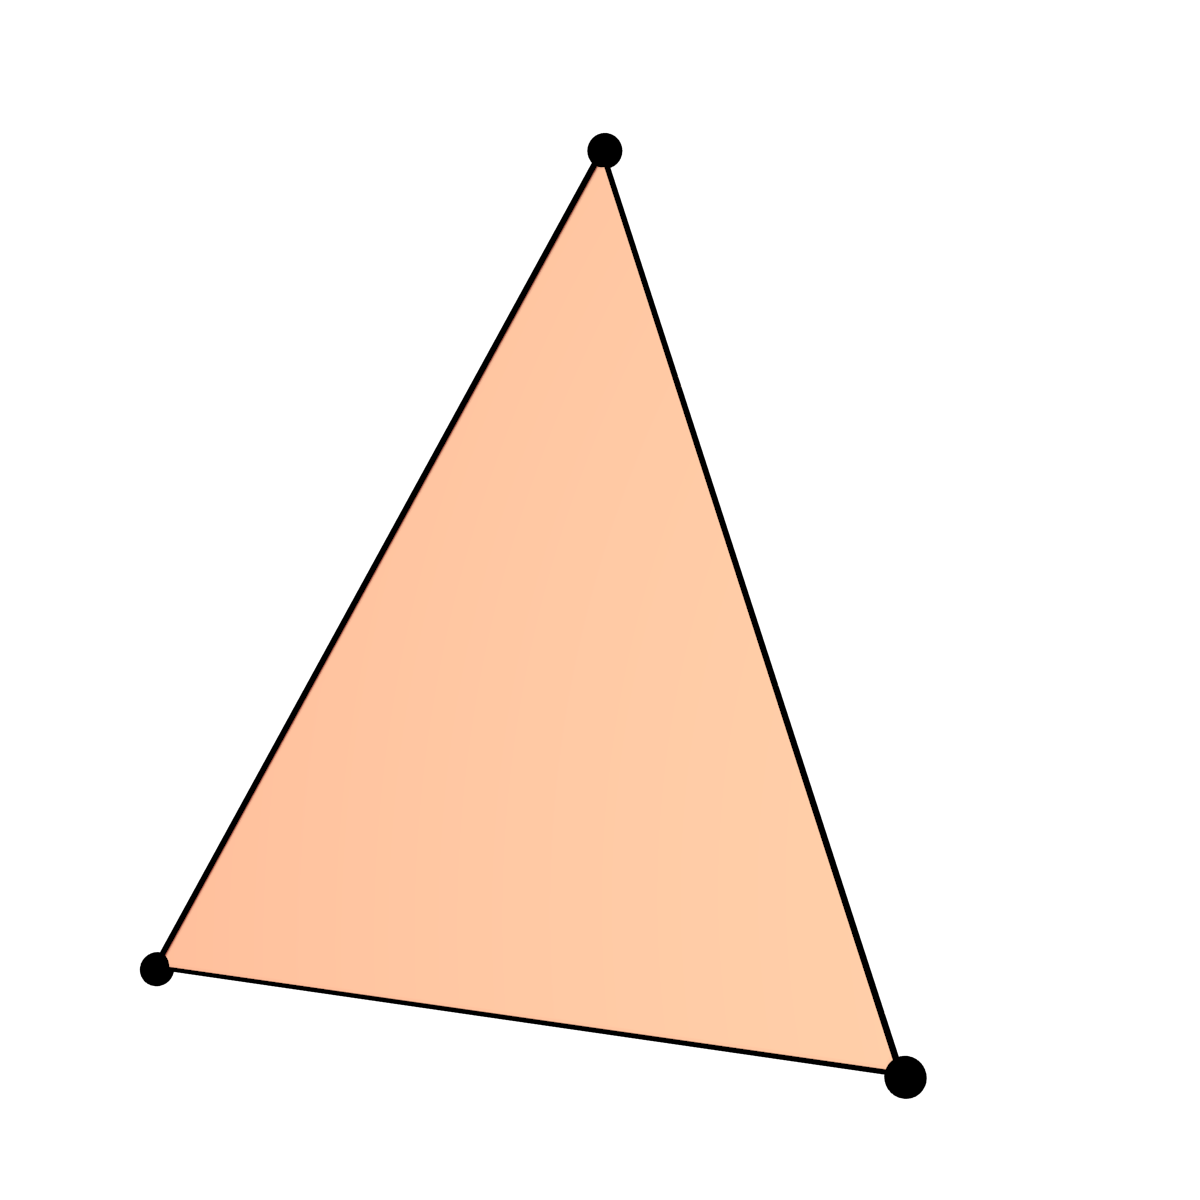
\includegraphics[width=0.9\textwidth]{./img/raw/gd-object-triangle.png}};
        
      \node (l1) at (1.25, -2.1) {$\mathbf{v_1}$};
      \node (l2) at (-1.75, -1.75) {$\mathbf{v_2}$};
      \node (l3) at (0, 2) {$\mathbf{v_3}$};
    \end{tikzpicture}
    \caption{Voorstelling van de driehoek $\bigtriangleup\mathbf{v_1}\mathbf{v_2}\mathbf{v_3}$}\label{fig:gd-object-tri}
  \end{subfigure} %
  \begin{subfigure}[b]{.6\linewidth}
    \centering
    \begin{tikzpicture}
      \node[inner sep=0pt] (img0) at (-0.25, 0.5)
           {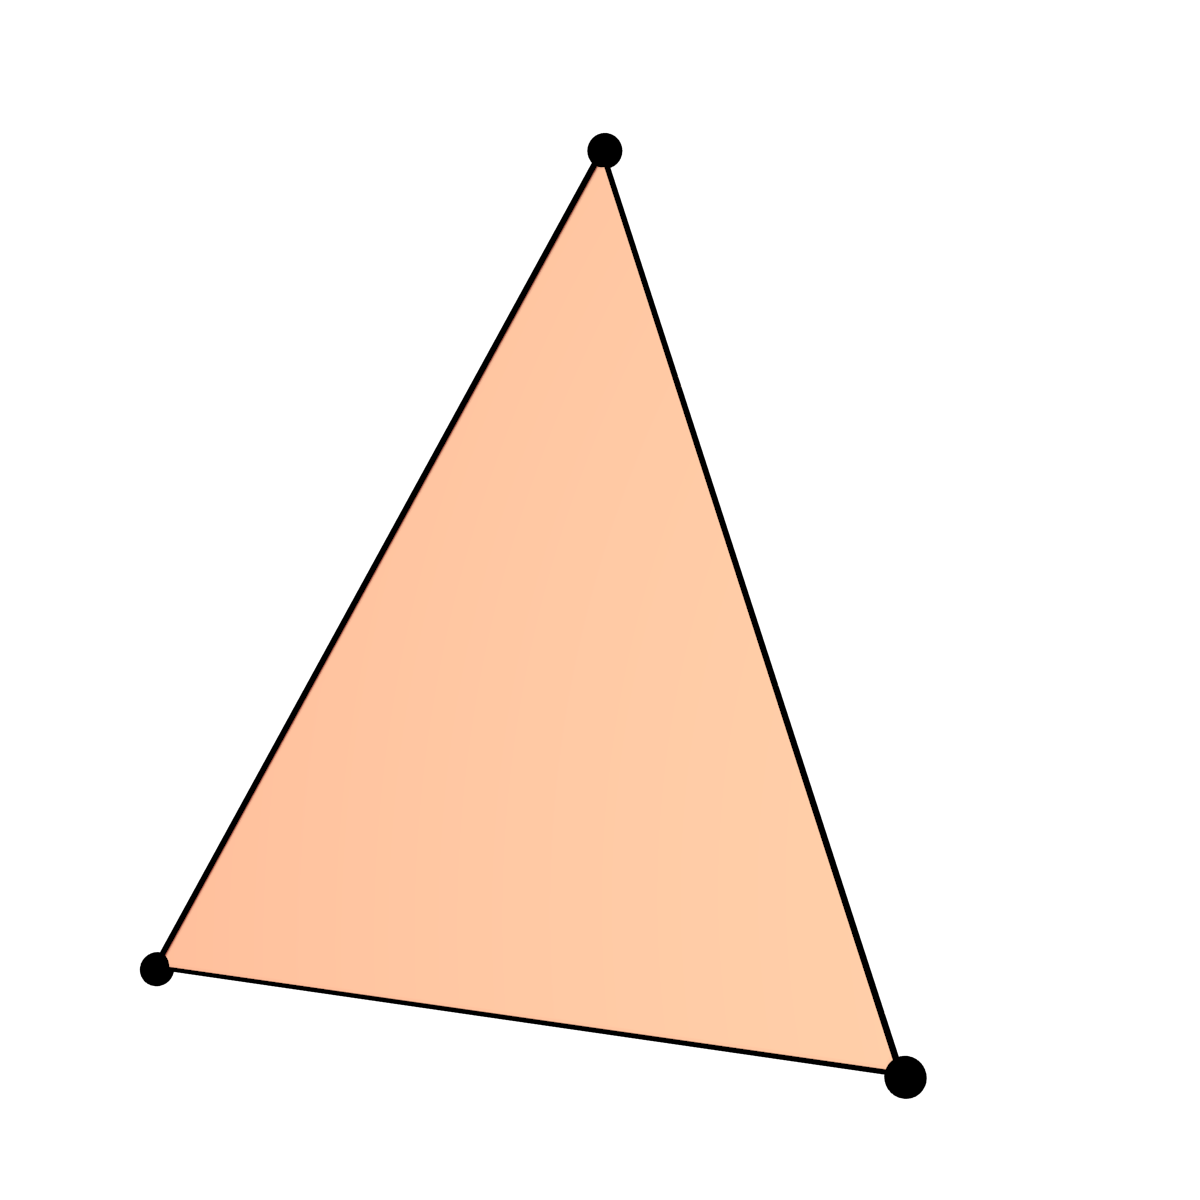
\includegraphics[width=0.35\textwidth]{./img/raw/gd-object-triangle.png}};
      \node[inner sep=0pt] (img1) at (0, 0)
           {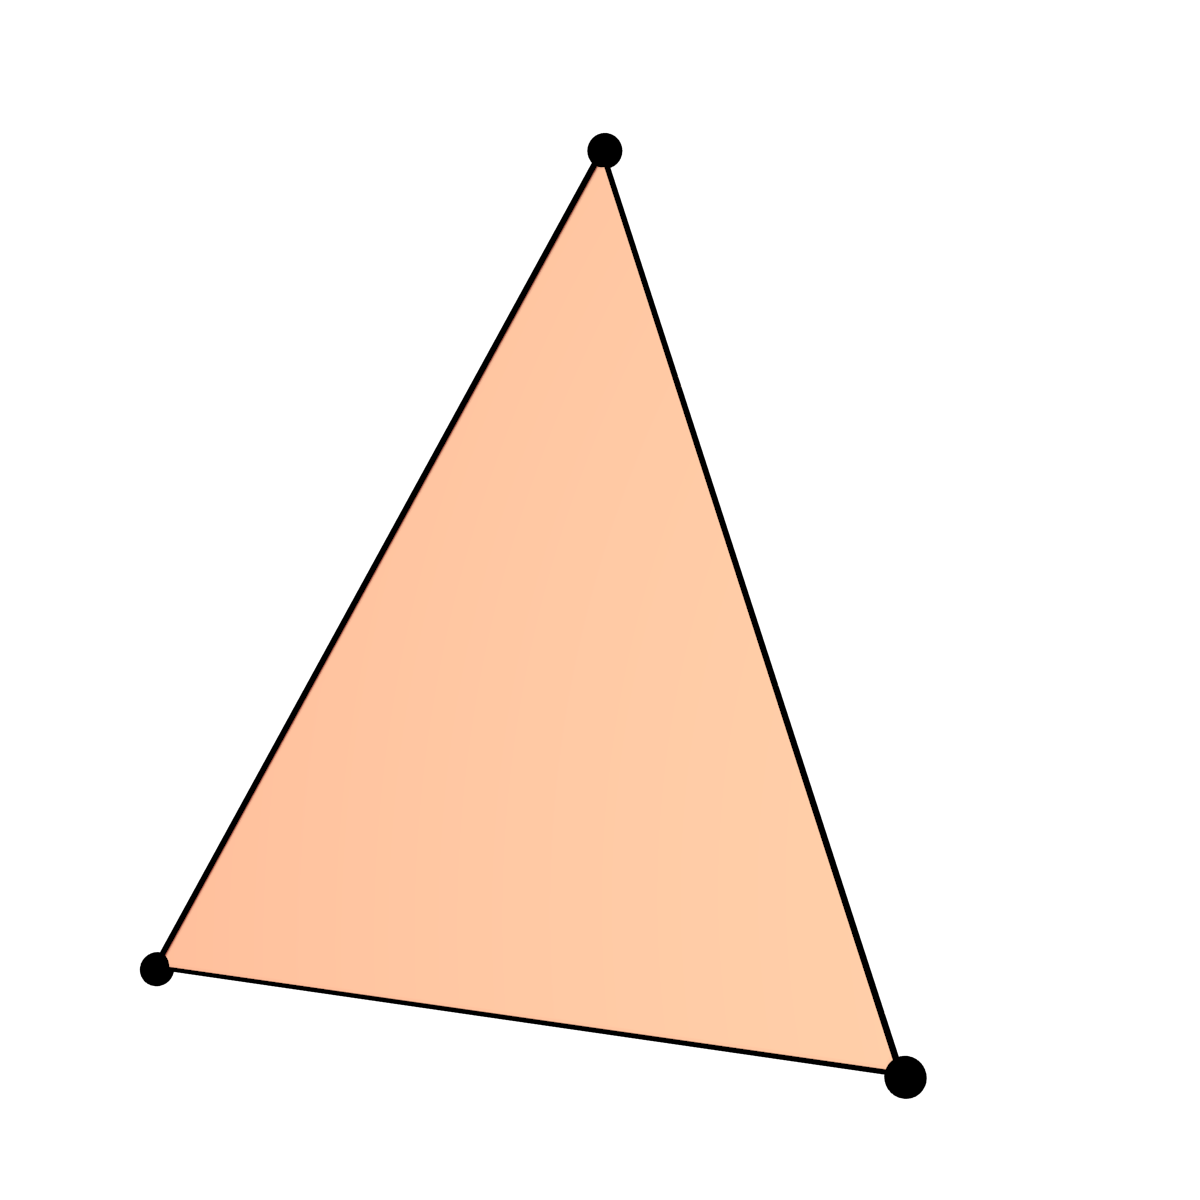
\includegraphics[width=0.35\textwidth]{./img/raw/gd-object-triangle.png}};
      \node[inner sep=0pt] (img2) at (0.25, -0.5)
           {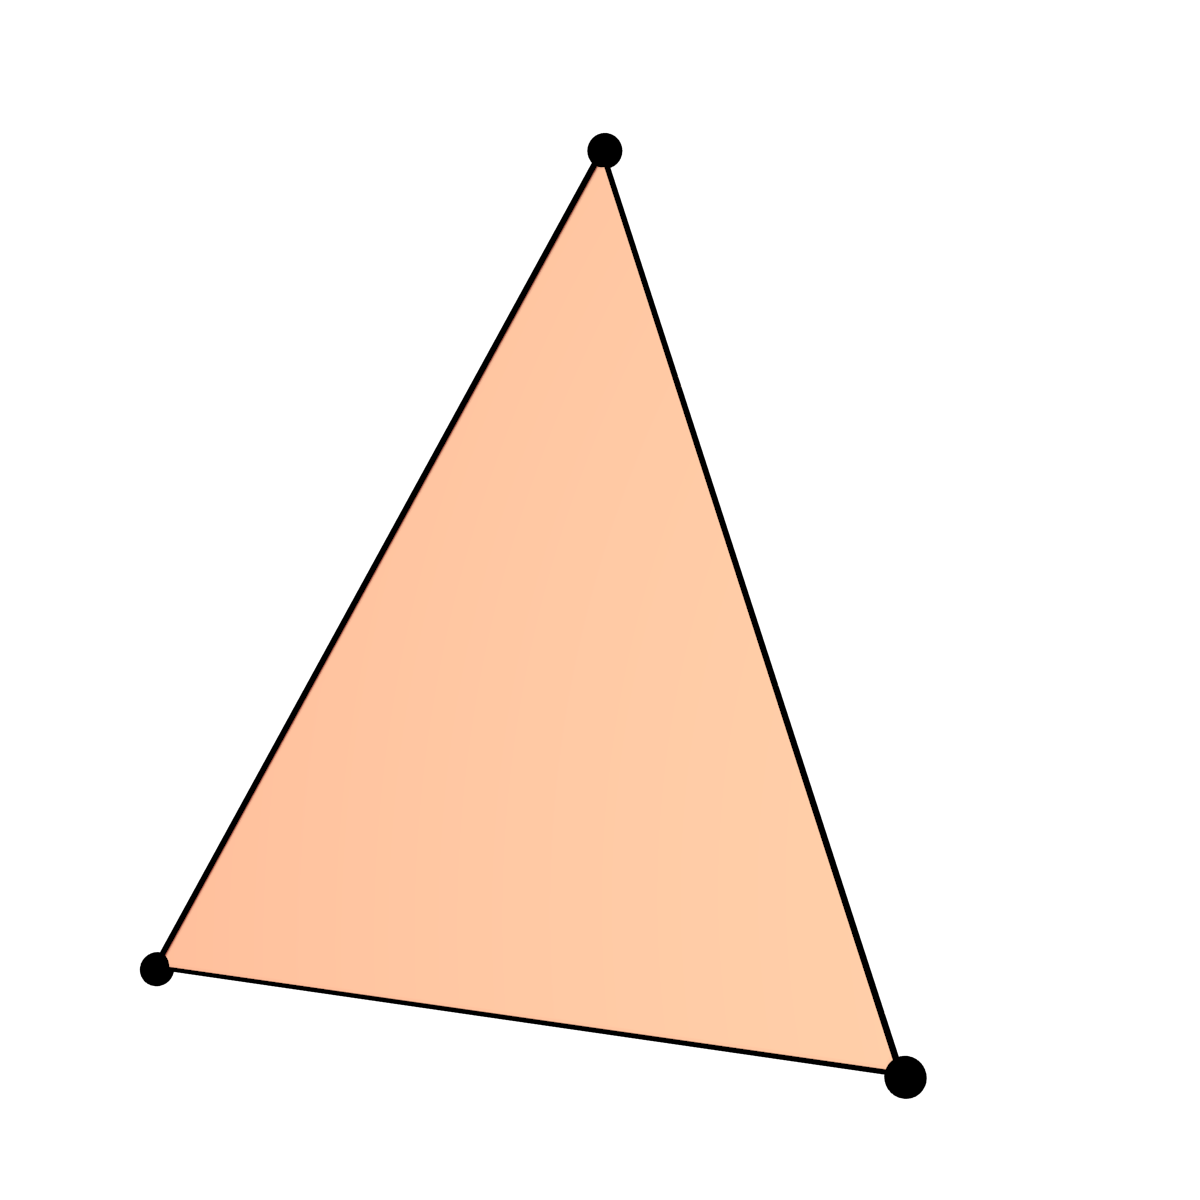
\includegraphics[width=0.35\textwidth]{./img/raw/gd-object-triangle.png}};

      \node[inner sep=0pt] (img3) at (5.0, 0.0)
           {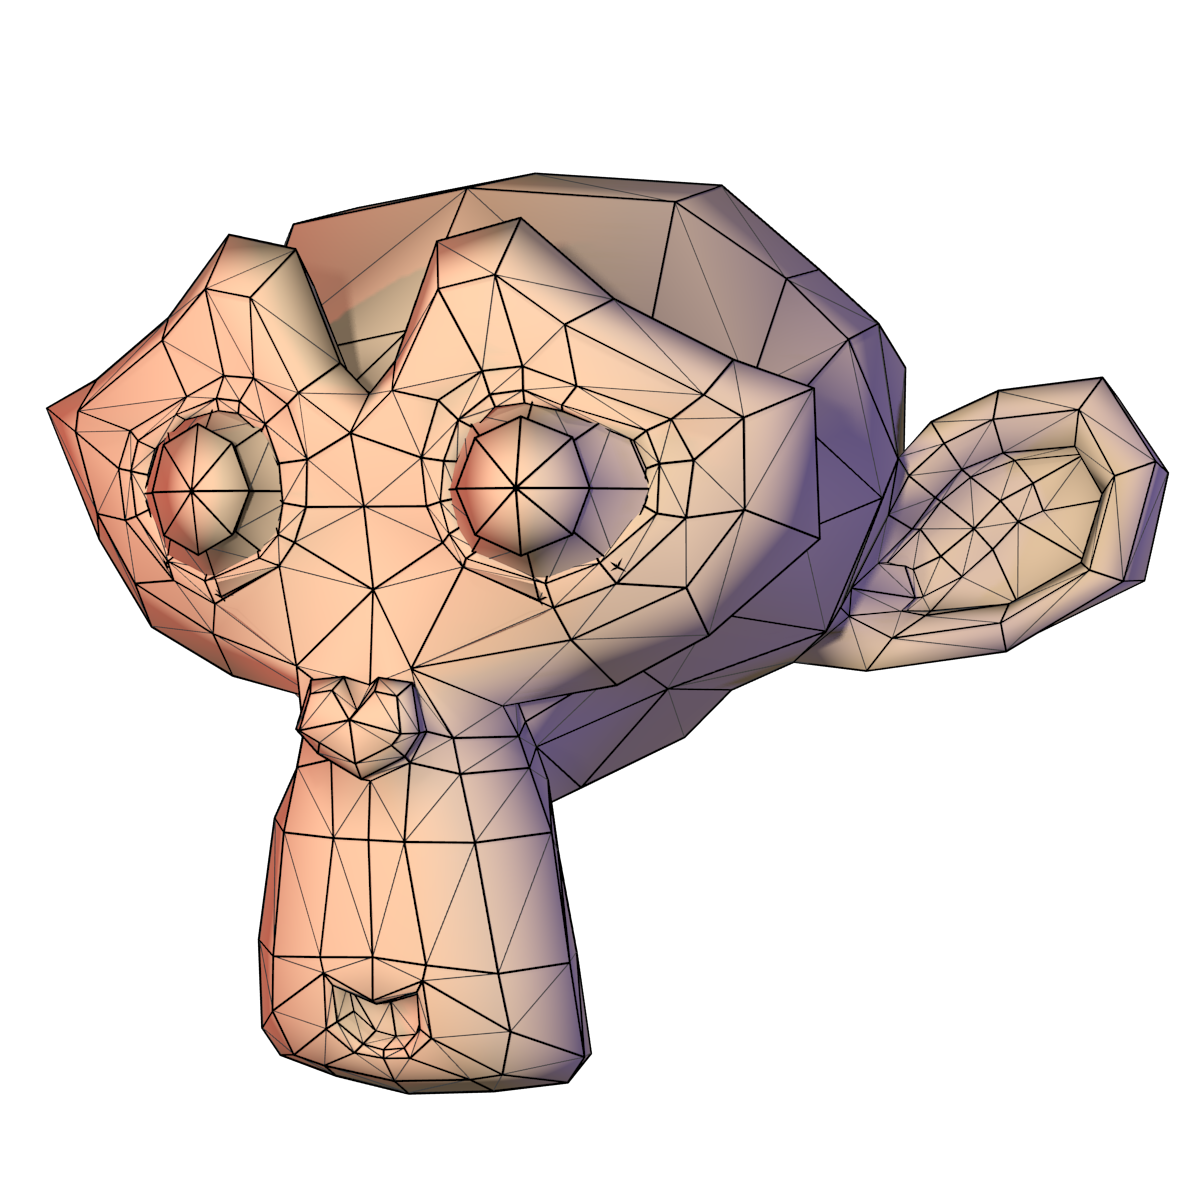
\includegraphics[width=0.625\textwidth]{./img/raw/gd-object-mesh.png}};
           
      \node (l3) at (0.25, -2.5) {Collectie van driehoeken};
      \draw[-stealth, thick] (1.5,0) -- (2.5,0);
    \end{tikzpicture}
    \caption{Voorstelling van een mesh als collectie van driehoeken.}\label{fig:gd-object-mesh}
  \end{subfigure}
  \\
    \begin{subfigure}[b]{.95\linewidth}
    \centering
    \begin{tikzpicture}
      \node[inner sep=0pt] (img1) at (0.0, -1.0)
           {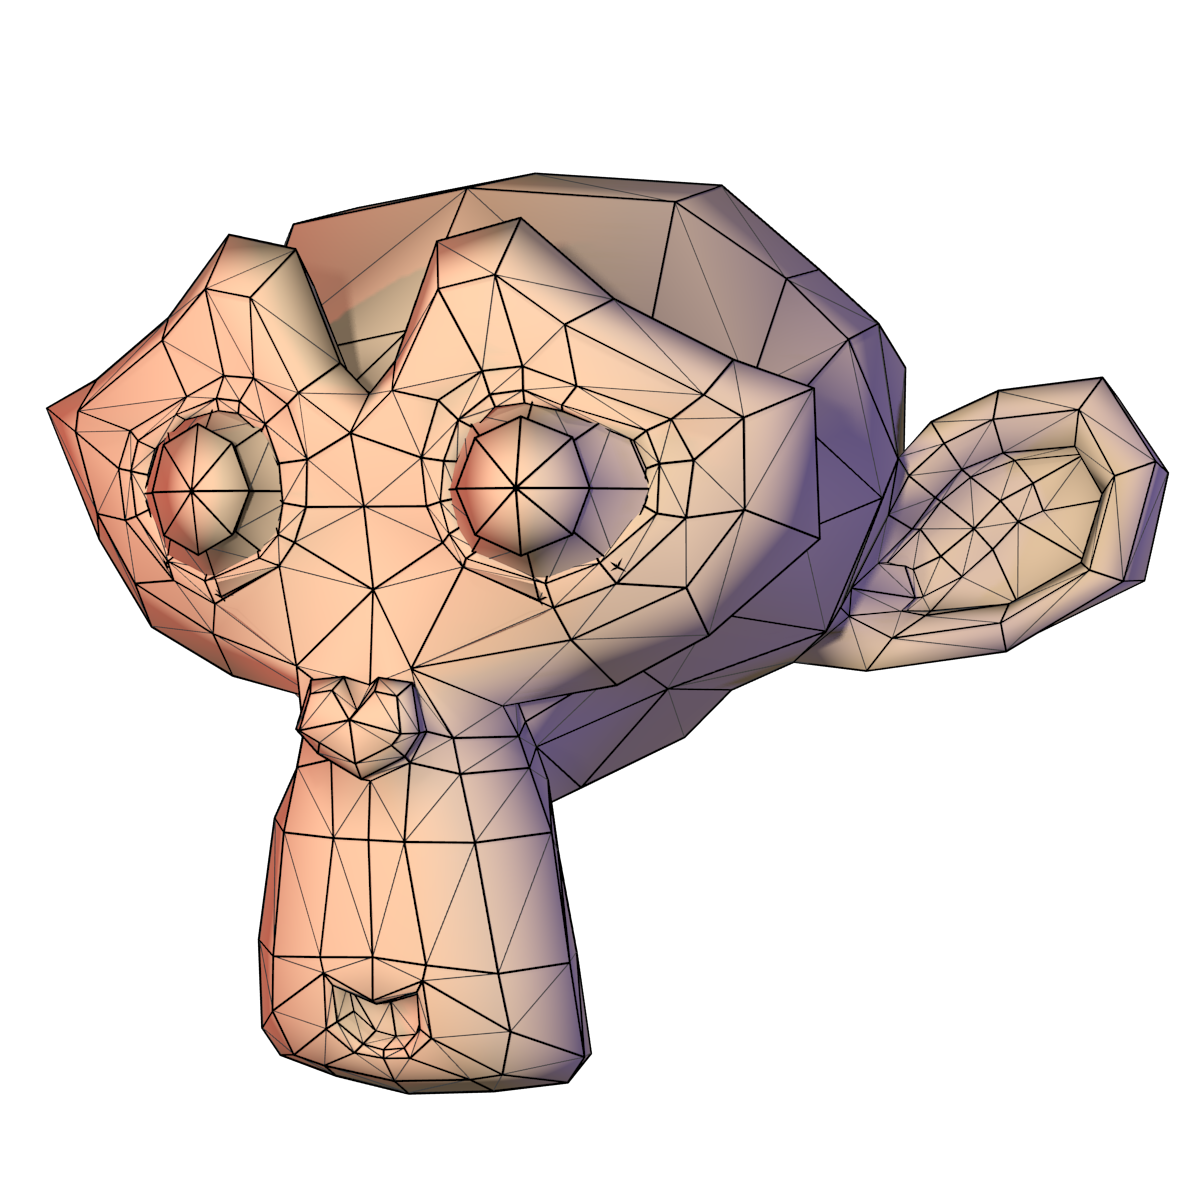
\includegraphics[width=0.25\textwidth]{./img/raw/gd-object-mesh.png}};
           \node (l2) at (0.0, -4) {Mesh};

           \node (l3) at (0.0, -5) {$\lbrace A_1, A_2, A_3, A_4 \rbrace$};
           \node (l3) at (0.0, -5.5) {\'E\'en transformatie matrix $A$ per object};
           %\node (l3) at (0.0, -5) {$\lbrace A_1, A_2, A_3, A_4 \rbrace \text{ where } A_i =
           %  \begin{bmatrix}
           %    a_{1,1} & a_{2,1} & a_{3,1} & a_{4, 1} \\
           %    a_{1,2} & a_{2,2} & a_{3,2} & a_{4, 2} \\
           %    a_{1,3} & a_{2,3} & a_{3,3} & a_{4, 3} \\
           %    a_{1,4} & a_{2,4} & a_{3,4} & a_{4, 4} \\
           %  \end{bmatrix}$};
           %\node (l3) at (0.0, -6.5) {\'E\'en transformatie matrix per object};

           \draw[-stealth, thick] (2.5,-4.5) -- (3.5,-4.5);
           \node[inner sep=0pt] (img1) at (7.5, -1.0)
                {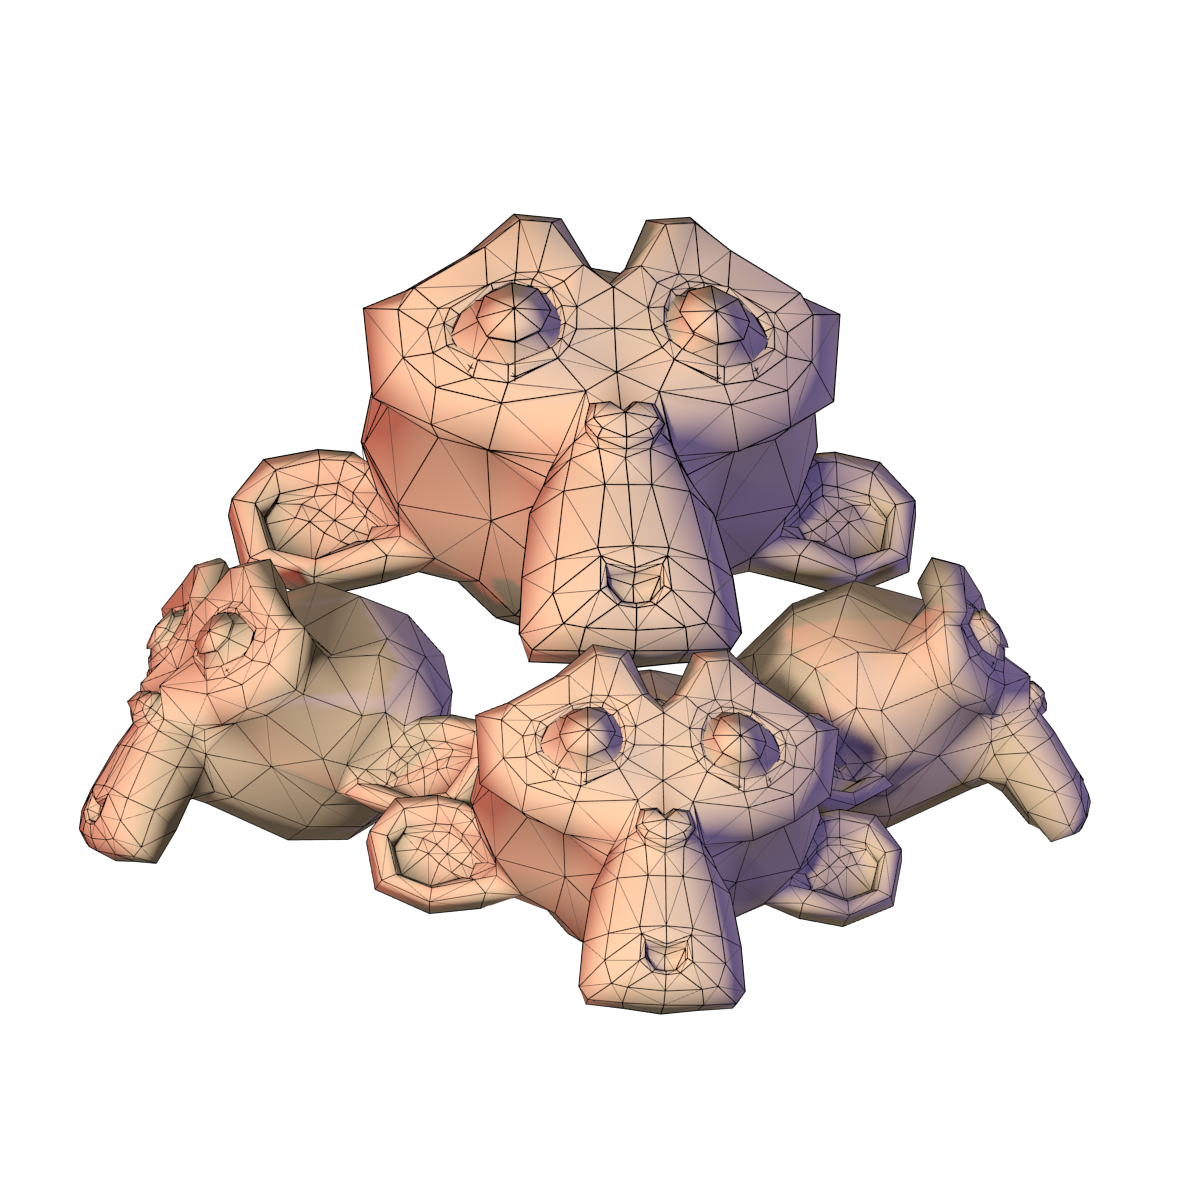
\includegraphics[width=0.65\textwidth]{./img/raw/gd-object-obj.png}};
           \node (l4) at (7.0, -5.5) {Collectie van objecten};
    \end{tikzpicture}
    \caption{Voorstelling van een set van objecten bestaande uit \'e\'en mesh en vier transformatie matrices.}\label{fig:gd-object-obj}
  \end{subfigure}
  \caption{Voorstelling van objecten doormiddel van driehoeken.}
  \label{fig:gd-object}
\end{figure}

